% Options for packages loaded elsewhere
\PassOptionsToPackage{unicode}{hyperref}
\PassOptionsToPackage{hyphens}{url}
%
\documentclass[
  a4paper,
]{scrbook}

\usepackage{amsmath,amssymb}
\usepackage{setspace}
\usepackage{iftex}
\ifPDFTeX
  \usepackage[T1]{fontenc}
  \usepackage[utf8]{inputenc}
  \usepackage{textcomp} % provide euro and other symbols
\else % if luatex or xetex
  \usepackage{unicode-math}
  \defaultfontfeatures{Scale=MatchLowercase}
  \defaultfontfeatures[\rmfamily]{Ligatures=TeX,Scale=1}
\fi
\usepackage{lmodern}
\ifPDFTeX\else  
    % xetex/luatex font selection
\fi
% Use upquote if available, for straight quotes in verbatim environments
\IfFileExists{upquote.sty}{\usepackage{upquote}}{}
\IfFileExists{microtype.sty}{% use microtype if available
  \usepackage[]{microtype}
  \UseMicrotypeSet[protrusion]{basicmath} % disable protrusion for tt fonts
}{}
\makeatletter
\@ifundefined{KOMAClassName}{% if non-KOMA class
  \IfFileExists{parskip.sty}{%
    \usepackage{parskip}
  }{% else
    \setlength{\parindent}{0pt}
    \setlength{\parskip}{6pt plus 2pt minus 1pt}}
}{% if KOMA class
  \KOMAoptions{parskip=half}}
\makeatother
\usepackage{xcolor}
\usepackage[left=2.54cm,right=2.54cm]{geometry}
\setlength{\emergencystretch}{3em} % prevent overfull lines
\setcounter{secnumdepth}{5}
% Make \paragraph and \subparagraph free-standing
\makeatletter
\ifx\paragraph\undefined\else
  \let\oldparagraph\paragraph
  \renewcommand{\paragraph}{
    \@ifstar
      \xxxParagraphStar
      \xxxParagraphNoStar
  }
  \newcommand{\xxxParagraphStar}[1]{\oldparagraph*{#1}\mbox{}}
  \newcommand{\xxxParagraphNoStar}[1]{\oldparagraph{#1}\mbox{}}
\fi
\ifx\subparagraph\undefined\else
  \let\oldsubparagraph\subparagraph
  \renewcommand{\subparagraph}{
    \@ifstar
      \xxxSubParagraphStar
      \xxxSubParagraphNoStar
  }
  \newcommand{\xxxSubParagraphStar}[1]{\oldsubparagraph*{#1}\mbox{}}
  \newcommand{\xxxSubParagraphNoStar}[1]{\oldsubparagraph{#1}\mbox{}}
\fi
\makeatother

\usepackage{color}
\usepackage{fancyvrb}
\newcommand{\VerbBar}{|}
\newcommand{\VERB}{\Verb[commandchars=\\\{\}]}
\DefineVerbatimEnvironment{Highlighting}{Verbatim}{commandchars=\\\{\}}
% Add ',fontsize=\small' for more characters per line
\usepackage{framed}
\definecolor{shadecolor}{RGB}{255,255,255}
\newenvironment{Shaded}{\begin{snugshade}}{\end{snugshade}}
\newcommand{\AlertTok}[1]{\textcolor[rgb]{0.75,0.01,0.01}{\textbf{\colorbox[rgb]{0.97,0.90,0.90}{#1}}}}
\newcommand{\AnnotationTok}[1]{\textcolor[rgb]{0.79,0.38,0.79}{#1}}
\newcommand{\AttributeTok}[1]{\textcolor[rgb]{0.00,0.34,0.68}{#1}}
\newcommand{\BaseNTok}[1]{\textcolor[rgb]{0.69,0.50,0.00}{#1}}
\newcommand{\BuiltInTok}[1]{\textcolor[rgb]{0.39,0.29,0.61}{\textbf{#1}}}
\newcommand{\CharTok}[1]{\textcolor[rgb]{0.57,0.30,0.62}{#1}}
\newcommand{\CommentTok}[1]{\textcolor[rgb]{0.54,0.53,0.53}{#1}}
\newcommand{\CommentVarTok}[1]{\textcolor[rgb]{0.00,0.58,1.00}{#1}}
\newcommand{\ConstantTok}[1]{\textcolor[rgb]{0.67,0.33,0.00}{#1}}
\newcommand{\ControlFlowTok}[1]{\textcolor[rgb]{0.12,0.11,0.11}{\textbf{#1}}}
\newcommand{\DataTypeTok}[1]{\textcolor[rgb]{0.00,0.34,0.68}{#1}}
\newcommand{\DecValTok}[1]{\textcolor[rgb]{0.69,0.50,0.00}{#1}}
\newcommand{\DocumentationTok}[1]{\textcolor[rgb]{0.38,0.47,0.50}{#1}}
\newcommand{\ErrorTok}[1]{\textcolor[rgb]{0.75,0.01,0.01}{\underline{#1}}}
\newcommand{\ExtensionTok}[1]{\textcolor[rgb]{0.00,0.58,1.00}{\textbf{#1}}}
\newcommand{\FloatTok}[1]{\textcolor[rgb]{0.69,0.50,0.00}{#1}}
\newcommand{\FunctionTok}[1]{\textcolor[rgb]{0.39,0.29,0.61}{#1}}
\newcommand{\ImportTok}[1]{\textcolor[rgb]{1.00,0.33,0.00}{#1}}
\newcommand{\InformationTok}[1]{\textcolor[rgb]{0.69,0.50,0.00}{#1}}
\newcommand{\KeywordTok}[1]{\textcolor[rgb]{0.12,0.11,0.11}{\textbf{#1}}}
\newcommand{\NormalTok}[1]{\textcolor[rgb]{0.12,0.11,0.11}{#1}}
\newcommand{\OperatorTok}[1]{\textcolor[rgb]{0.12,0.11,0.11}{#1}}
\newcommand{\OtherTok}[1]{\textcolor[rgb]{0.00,0.43,0.16}{#1}}
\newcommand{\PreprocessorTok}[1]{\textcolor[rgb]{0.00,0.43,0.16}{#1}}
\newcommand{\RegionMarkerTok}[1]{\textcolor[rgb]{0.00,0.34,0.68}{\colorbox[rgb]{0.88,0.91,0.97}{#1}}}
\newcommand{\SpecialCharTok}[1]{\textcolor[rgb]{0.24,0.68,0.91}{#1}}
\newcommand{\SpecialStringTok}[1]{\textcolor[rgb]{1.00,0.33,0.00}{#1}}
\newcommand{\StringTok}[1]{\textcolor[rgb]{0.75,0.01,0.01}{#1}}
\newcommand{\VariableTok}[1]{\textcolor[rgb]{0.00,0.34,0.68}{#1}}
\newcommand{\VerbatimStringTok}[1]{\textcolor[rgb]{0.75,0.01,0.01}{#1}}
\newcommand{\WarningTok}[1]{\textcolor[rgb]{0.75,0.01,0.01}{#1}}

\providecommand{\tightlist}{%
  \setlength{\itemsep}{0pt}\setlength{\parskip}{0pt}}\usepackage{longtable,booktabs,array}
\usepackage{calc} % for calculating minipage widths
% Correct order of tables after \paragraph or \subparagraph
\usepackage{etoolbox}
\makeatletter
\patchcmd\longtable{\par}{\if@noskipsec\mbox{}\fi\par}{}{}
\makeatother
% Allow footnotes in longtable head/foot
\IfFileExists{footnotehyper.sty}{\usepackage{footnotehyper}}{\usepackage{footnote}}
\makesavenoteenv{longtable}
\usepackage{graphicx}
\makeatletter
\newsavebox\pandoc@box
\newcommand*\pandocbounded[1]{% scales image to fit in text height/width
  \sbox\pandoc@box{#1}%
  \Gscale@div\@tempa{\textheight}{\dimexpr\ht\pandoc@box+\dp\pandoc@box\relax}%
  \Gscale@div\@tempb{\linewidth}{\wd\pandoc@box}%
  \ifdim\@tempb\p@<\@tempa\p@\let\@tempa\@tempb\fi% select the smaller of both
  \ifdim\@tempa\p@<\p@\scalebox{\@tempa}{\usebox\pandoc@box}%
  \else\usebox{\pandoc@box}%
  \fi%
}
% Set default figure placement to htbp
\def\fps@figure{htbp}
\makeatother
% definitions for citeproc citations
\NewDocumentCommand\citeproctext{}{}
\NewDocumentCommand\citeproc{mm}{%
  \begingroup\def\citeproctext{#2}\cite{#1}\endgroup}
\makeatletter
 % allow citations to break across lines
 \let\@cite@ofmt\@firstofone
 % avoid brackets around text for \cite:
 \def\@biblabel#1{}
 \def\@cite#1#2{{#1\if@tempswa , #2\fi}}
\makeatother
\newlength{\cslhangindent}
\setlength{\cslhangindent}{1.5em}
\newlength{\csllabelwidth}
\setlength{\csllabelwidth}{3em}
\newenvironment{CSLReferences}[2] % #1 hanging-indent, #2 entry-spacing
 {\begin{list}{}{%
  \setlength{\itemindent}{0pt}
  \setlength{\leftmargin}{0pt}
  \setlength{\parsep}{0pt}
  % turn on hanging indent if param 1 is 1
  \ifodd #1
   \setlength{\leftmargin}{\cslhangindent}
   \setlength{\itemindent}{-1\cslhangindent}
  \fi
  % set entry spacing
  \setlength{\itemsep}{#2\baselineskip}}}
 {\end{list}}
\usepackage{calc}
\newcommand{\CSLBlock}[1]{\hfill\break\parbox[t]{\linewidth}{\strut\ignorespaces#1\strut}}
\newcommand{\CSLLeftMargin}[1]{\parbox[t]{\csllabelwidth}{\strut#1\strut}}
\newcommand{\CSLRightInline}[1]{\parbox[t]{\linewidth - \csllabelwidth}{\strut#1\strut}}
\newcommand{\CSLIndent}[1]{\hspace{\cslhangindent}#1}

% Palatino font:
\usepackage[T1]{fontenc}
\usepackage[utf8]{inputenc}
\usepackage{palatino}

\usepackage{mathpazo}

\usepackage{upquote}

% front page
\usepackage[colorlinks]{hyperref} % for text color on title
\usepackage{titling} % makes \thetitle etc available...
\usepackage{lipsum}
\usepackage{tikz}
\tikzstyle{bag} = [align=center] % allows new lines in text below
\AtBeginDocument{\thispagestyle{empty}
\definecolor{titlecolor}{HTML}{1C2404}
\begin{tikzpicture}[remember picture,overlay]
\draw (current page.center) node[inner sep=0] {\resizebox{!}{350mm}{\includegraphics{highres_banner.pdf}}};
\draw (current page.center) node[inner sep=0, opacity=0.5] {\resizebox{!}{100mm}{
\includegraphics{ausegl_sort.pdf}}};
% \draw (current page.center) node[bag] {  
        \draw (17, 1.7) node[bag, align=right, anchor=north east] {  
    % \mytitlefont 
    \color{titlecolor} \Large \textbf{Thesis} \\ 
    \\ 
    % \mytitlefont 
    \color{titlecolor} \Huge \textbf{\thetitle} \\ 
    \\ 
    % \mytitlefont
    \color{titlecolor} \huge \theauthor \\
    \\
    % \mytitlefont 
    \color{titlecolor} \Large \thedate 
    };
\end{tikzpicture}
\clearpage}

% back side
\AtEndDocument{\clearpage\thispagestyle{empty}
\begin{tikzpicture}[remember picture,overlay]
\draw (current page.center) node[inner sep=0] {\resizebox{!}{350mm}{\includegraphics{highres_banner.pdf}}};
% \draw (current page.center) node[bag] {  
    \draw (17, 1.7) node[bag, align=right, anchor=north east] {  
        % \mytitlefont 
        \color{titlecolor} \large Bioinformatics Research Centre \\ 
        % \mytitlefont 
        \color{titlecolor} \large Department of Molecular Biology and Genetics \\ 
        % \mytitlefont 
        \color{titlecolor} \large Aarhus University \\
        % \mytitlefont 
        \color{titlecolor} \large Universitetsbyen 81 \\
        % \mytitlefont 
        \color{titlecolor} \large 8000 Aarhus C \\
        % \mytitlefont 
        \color{titlecolor} \large Denmark
        };

\end{tikzpicture}}


% % picture (AU logo in title page)
% \usepackage{titlepic}
% % \usepackage{graphicx}
% \titlepic{\resizebox{!}{50mm}{
\includegraphics[width=\textwidth]{ausegl_sort.pdf}}}



% \pagestyle{plain} % no running header

\usepackage[many]{tcolorbox}
\definecolor{quotegray}{HTML}{505050}
\newtcolorbox{myquote}{%
    enhanced jigsaw, 
    breakable,      % allow page breaks
    frame hidden,   % hide the default frame
    left=1cm,       % left margin
    right=1cm,      % right margin
    colback=white,
    fontupper=\color{quotegray},
    overlay={%
        \node [scale=4,
            text=lightgray,
            inner sep=0pt,] at ([xshift=0.5cm,yshift=-0.7cm]frame.north west){``}; 
        \node [scale=4,
            text=lightgray,
            inner sep=0pt,] at ([xshift=-0.5cm]frame.south east){''};  
            },
        % paragraph skips obeyed within tcolorbox
                parbox=false,
}
% redefine the 'quote' environment to use this 'myquote' environment
\renewenvironment{quote}{\begin{myquote}}{\end{myquote}}

% add a dummy abstract environment that is defined in quarto manuscript 
% but not in the quarto book that we run first to give it a slot in the 
% side bar
\ifcsmacro{abstract}{}{
  \let\endmyenvironment\undefined%
  \newenvironment{abstract}{\chapter*{Abstract}}{}
}

% \usepackage{framed} % not sure i need this anymore

% \usepackage[T1]{fontenc}
% \usepackage{inconsolata}

% % I have to only define Shaded if it is already defined.
% % The reason is that pandoc does not define the macro if there are not code blocks in the a markdown file.
% \ifx \@Shaded \@empty

% \renewcommand{\KeywordTok}[1]{\textcolor[rgb]{0, 0, 0}{\textbf{{#1}}}} % def and or not reg
% \renewcommand{\BuiltInTok}[1]{\textcolor[rgb]{0.373, 0.298, 0.580}{\textbf{{#1}}}} % print open 
% \renewcommand{\VariableTok}[1]{\textcolor[rgb]{0.141, 0.392, 0.824}{\textbf{{#1}}}}
% \renewcommand{\OperatorTok}[1]{\textcolor[rgb]{0, 0, 0}{{#1}}} % def and or not reg
% \renewcommand{\DataTypeTok}[1]{\textcolor[rgb]{1.0,0.13,0.00}{{#1}}}
% \renewcommand{\DecValTok}[1]{\textcolor[rgb]{0.655, 0.498, 0.161}{{#1}}}
% \renewcommand{\BaseNTok}[1]{\textcolor[rgb]{0.259, 0.592, 0.596}{{#1}}}
% \renewcommand{\FloatTok}[1]{\textcolor[rgb]{0.655, 0.498, 0.161}{{#1}}}
% \renewcommand{\CharTok}[1]{\textcolor[rgb]{0.678,0.141,0.098}{{#1}}}
% \renewcommand{\StringTok}[1]{\textcolor[rgb]{0.678,0.141,0.098}{{#1}}}
% \renewcommand{\CommentTok}[1]{\textcolor[rgb]{0.135, 0.134, 0.133}{{#1}}}
% \renewcommand{\OtherTok}[1]{\textcolor[rgb]{0.00,0.44,0.13}{{#1}}}
% \renewcommand{\AlertTok}[1]{\textcolor[rgb]{1.00,0.00,0.00}{\textbf{{#1}}}}
% \renewcommand{\FunctionTok}[1]{\textcolor[rgb]{0.549, 0.102, 0.063}{\textbf{{#1}}}}  % function name
% \renewcommand{\RegionMarkerTok}[1]{{#1}}
% \renewcommand{\ErrorTok}[1]{\textcolor[rgb]{1.00,0.00,0.00}{\textbf{{#1}}}}
% \renewcommand{\NormalTok}[1]{\textcolor[rgb]{0, 0, 0}{{#1}}}


% \else
%   % no code blocks with markup...
% \fi



\usepackage{etoolbox}
\makeatletter
\g@addto@macro{\appendix}{%
  \patchcmd{\@@makechapterhead}% <cmd>
    {\endgraf\nobreak\vskip.5\baselineskip}% <search>
    {\hspace*{-.5em}:\space}% <replace>
    {}{}% <success><failure>
  \patchcmd{\@chapter}% <cmd>
    {\addchaptertocentry{\thechapter}}% <search>
    {\addchaptertocentry{Appendix~\thechapter:}}% <replace>
    {}{}% <success><failure>
  \addtocontents{toc}{%
    \protect\patchcmd{\protect\l@chapter}% <cmd>
      {1.5em}% <search>
      {6.5em}% <replace>
      {}{}}% <success><failure>
}
\renewcommand{\autodot}{}% Remove all end-of-counter dots
\makeatother


% restart chapter numbers in each part
\makeatletter
\@addtoreset{chapter}{part}
\makeatother


% \usepackage{chngcntr}
% \counterwithin*{subsubsection}{chapter}
% \counterwithout*{subsubsection}{section}
% \counterwithout*{subsubsection}{subsection}

% %  % KMT only use subsubsection number (this increments though the book 
% %  % when we supress numbering with  {.unnumbered} after each header except Exerisices
% \renewcommand\thesubsubsection{\arabic{section}}
% \renewcommand\thesubsubsection{\arabic{subsection}}
% \renewcommand\thesubsubsection{\arabic{chapter}-\arabic{subsubsection}}


\renewcommand*{\chapterformat}{%
\textcolor[rgb]{0.7, 0.7, 0.7}{\thechapter}\autodot\enskip%
}
\renewcommand*{\sectionformat}{%
\textcolor[rgb]{0.7, 0.7, 0.7}{\thesection}\autodot\enskip%
}
\renewcommand*{\subsectionformat}{%
\textcolor[rgb]{0.7, 0.7, 0.7}{\thesubsection}\autodot\enskip%
}
\renewcommand*{\subsubsectionformat}{%
\textcolor[rgb]{0.7, 0.7, 0.7}{\thesubsubsection}\autodot\enskip%
}



% % prevent latex from "floating" the figures
% \usepackage{float}
% \let\origfigure\figure
% \let\endorigfigure\endfigure
% \renewenvironment{figure}[1][2] {
%     \expandafter\origfigure\expandafter[H]
% } {
%     \endorigfigure
% }

\usepackage{xcolor}
% \let\oldtextit\textit 
% \renewcommand\textit[1]{\oldtextit{\color{blue}#1}}
\let\oldemph\emph
\renewcommand\emph[1]{\oldemph{\color{gray}#1}}

\makeatletter
\@ifpackageloaded{caption}{}{\usepackage{caption}}
\AtBeginDocument{%
\ifdefined\contentsname
  \renewcommand*\contentsname{Table of contents}
\else
  \newcommand\contentsname{Table of contents}
\fi
\ifdefined\listfigurename
  \renewcommand*\listfigurename{List of Figures}
\else
  \newcommand\listfigurename{List of Figures}
\fi
\ifdefined\listtablename
  \renewcommand*\listtablename{List of Tables}
\else
  \newcommand\listtablename{List of Tables}
\fi
\ifdefined\figurename
  \renewcommand*\figurename{Figure}
\else
  \newcommand\figurename{Figure}
\fi
\ifdefined\tablename
  \renewcommand*\tablename{Table}
\else
  \newcommand\tablename{Table}
\fi
}
\@ifpackageloaded{float}{}{\usepackage{float}}
\floatstyle{ruled}
\@ifundefined{c@chapter}{\newfloat{codelisting}{h}{lop}}{\newfloat{codelisting}{h}{lop}[chapter]}
\floatname{codelisting}{Listing}
\newcommand*\listoflistings{\listof{codelisting}{List of Listings}}
\makeatother
\makeatletter
\makeatother
\makeatletter
\@ifpackageloaded{caption}{}{\usepackage{caption}}
\@ifpackageloaded{subcaption}{}{\usepackage{subcaption}}
\makeatother

\usepackage{bookmark}

\IfFileExists{xurl.sty}{\usepackage{xurl}}{} % add URL line breaks if available
\urlstyle{same} % disable monospaced font for URLs
\hypersetup{
  pdftitle={Title of my thesis},
  pdfkeywords={Vestibulum, Nunc ac dignissim, Proin feugiat},
  hidelinks,
  pdfcreator={LaTeX via pandoc}}


\title{Title of my thesis}
\usepackage{etoolbox}
\makeatletter
\providecommand{\subtitle}[1]{% add subtitle to \maketitle
  \apptocmd{\@title}{\par {\large #1 \par}}{}{}
}
\makeatother
\subtitle{Some subtitle for my thesis}
\author{Your Name}
\date{November 27, 2024}

\begin{document}
\frontmatter
\cleardoublepage
\thispagestyle{empty}
{\centering
\hbox{}\vskip 0cm plus 1fill

{%\mytitlefont 
\Huge\bfseries Title of my thesis \par}
\vspace{3ex}
{\Large\bfseries Some subtitle for my thesis \par}
\vspace{6ex}

    {\Large\bfseries Your Name \par}
    %
        %
        {\bfseries\large Aarhus University \par}
    %
%
\vskip 0cm plus 2fill

{\resizebox{!}{50mm}{
\includegraphics[width=\textwidth]{ausegl_sort.pdf}} \par}
\vskip 0cm plus 2fill

{\bfseries\Large\textit{Master of Science in Bioinformatics} \par}
\vspace{3ex}

{\bfseries\large November 27, 2024 \par}
\vspace{3ex}

\vspace{12ex}
{\small Submitted in fulfillment of the requirements
of the degree of Master of Science in Bioinformatics \par}
\pagebreak

\begin{quote}
\raggedright    
In plain language, the thesis describes an analysis of something.
Somethings was not previously know. I found something and was able to
conclude something. The perspectives of this result is something. \par
\raggedleft    
    {- Your Name \par}
%    
\end{quote}
}

\renewcommand*\contentsname{Table of contents}
{
\setcounter{tocdepth}{1}
\tableofcontents
}

\setstretch{1}
\mainmatter
\chapter{Introduction}\label{introduction}

\emph{Fringilla sem fusce vivamus pellentesque in commodo penatibus
bibendum. Vestibulum aptent volutpat vehicula eu rutrum lobortis
consequat. Euismod lectus ultrices; duis duis ipsum rhoncus. Ipsum vitae
primis potenti suscipit per nascetur rutrum lobortis. Scelerisque
pulvinar duis interdum sapien elementum consequat vitae orci.
Suspendisse tempor nisl accumsan dolor potenti euismod sed.}

\subsection{Subsection (with
references)}\label{subsection-with-references}

Skov et al.~reported strong selection on the human X chromosome (2023).
\emph{Pellentesque id tellus at erat luctus fringilla. Suspendisse
potenti. In fringilla gravida ornare. Aenean id lectus pulvinar,
sagittis felis nec, rutrum risus. Nam vel neque eu arcu blandit
fringilla et in quam. Aliquam luctus est sit amet vestibulum eleifend.}
Lineages in small population have smaller coalescence times, (see
Nielsen and Slatkin 2016, chap. 1). \emph{Nunc ac dignissim magna.
Vestibulum vitae egestas elit. Proin feugiat leo quis ante condimentum,
eu ornare mauris feugiat. Pellentesque habitant morbi tristique senectus
et netus et malesuada fames ac turpis egestas. Mauris cursus laoreet ex,
ignissim bibendum est posuere iaculis. Suspendisse et maximus elit.} The
neanderthal genome has been sequenced (Prüfer et al. 2012). \emph{Nunc
ac dignissim magna. Vestibulum vitae egestas elit. Proin feugiat leo
quis ante condimentum, eu ornare mauris feugiat.} The X chromosome is
subject to recurrent sweeps (Nam et al. 2015; Dutheil et al. 2015).
\emph{Fusce et ellentesque ligula. Pellentesque id tellus at erat luctus
fringilla. Suspendisse potenti. Pellentesque habitant morbi tristique
senectus et netus et malesuada fames ac turpis egestas.} Following Munch
et al. (2014), *dignissim magna. Vestibulum vitae egestas elit. Proin
feugiat leo quis ante condimentum, eu ornare mauris feugiat.

\subsection{Subsubsection (with
illustrations)}\label{subsubsection-with-illustrations}

\emph{In fringilla gravida ornare. Aenean id lectus pulvinar, sagittis
felis nec, rutrum risus. Nam vel neque eu arcu blandit fringilla et in
quam. Aliquam luctus est sit amet vestibulum eleifend.} You can see an
elephant in Figure~\ref{fig-elephant}. \emph{Phasellus elementum
sagittis molestie. Proin tempor lorem arcu, at condimentum purus
volutpat eu. Fusce et ellentesque ligula. Pellentesque id tellus at erat
luctus fringilla. Suspendisse potenti.}

\begin{figure}

\centering{

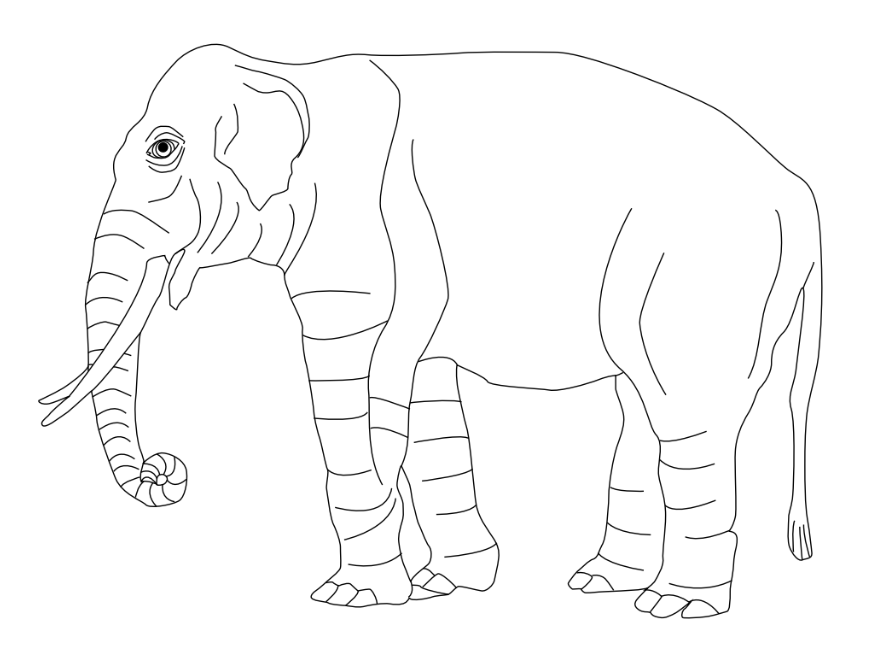
\includegraphics[width=0.5\linewidth,height=\textheight,keepaspectratio]{illustrations/elephant.png}

}

\caption{\label{fig-elephant}Some caption for an illustration showing an
elephant}

\end{figure}%

\emph{Integer vulputate habitant quis vitae tristique.Aenean id lectus
pulvinar, sagittis felis nec, rutrum risus. Nam vel neque eu arcu
blandit fringilla et in quam. Aliquam luctus est sit amet vestibulum
eleifend. Phasellus elementum sagittis molestie. Proin tempor lorem
arcu, at condimentum purus volutpat eu. Fusce et ellentesque ligula.}
There are two elephants in Figure~\ref{fig-twoelephants}.
\emph{Pellentesque id tellus at erat luctus fringilla. Suspendisse
potenti.} You can see an elephant in Figure~\ref{fig-elephant}.

\begin{figure}

\begin{minipage}{0.50\linewidth}

\centering{

\pandocbounded{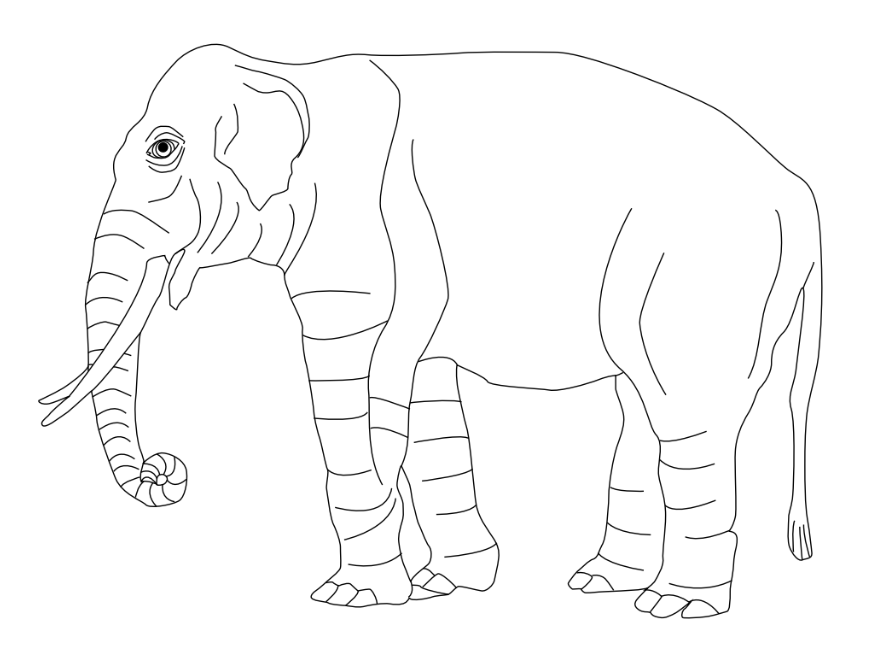
\includegraphics[keepaspectratio]{illustrations/elephant.png}}

}

\subcaption{\label{fig-surus}}

\end{minipage}%
%
\begin{minipage}{0.50\linewidth}

\centering{

\pandocbounded{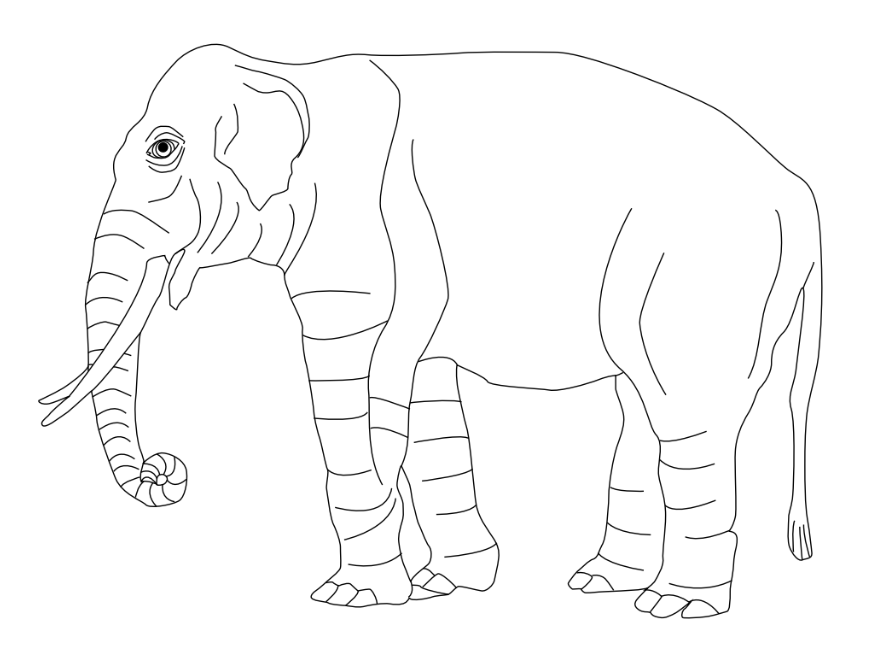
\includegraphics[keepaspectratio]{illustrations/elephant.png}}

}

\subcaption{\label{fig-hanno}}

\end{minipage}%

\caption{\label{fig-twoelephants}Some caption for an illustration with
two elephants.}

\end{figure}%

\chapter{Methods}\label{methods}

\emph{Nam senectus ultricies class nulla primis mattis. Primis feugiat
nunc nec in a bibendum elit; vestibulum molestie. Luctus vehicula
euismod fermentum semper facilisis. Integer vulputate habitant quis
vitae tristique. Fringilla sem fusce vivamus pellentesque in commodo
penatibus bibendum. Vestibulum aptent volutpat vehicula eu rutrum
lobortis consequat. Scelerisque pulvinar duis interdum sapien elementum
consequat vitae orci. Suspendisse tempor nisl accumsan dolor potenti
euismod sed.}

\section{Subsection (with text from
notebook)}\label{subsection-with-text-from-notebook}

\phantomsection\label{doc-sampling}
The 24 subjects from workplaces in Denmark were interviewed \ldots. blah
blah blah blah blah blah blah blah blah blah blah blah blah blah blah
blah blah blah blah blah blah blah blah blah blah blah blah blah blah
blah blah blah blah blah blah blah

\emph{Euismod lectus ultrices; duis duis ipsum rhoncus. Ipsum vitae
primis potenti suscipit per nascetur rutrum lobortis. Suspendisse et
maximus elit. In fringilla gravida ornare. Aenean id lectus pulvinar,
sagittis felis nec, rutrum risus. Nam vel neque eu arcu blandit
fringilla et in quam. Aliquam luctus est sit amet vestibulum eleifend.
Phasellus elementum sagittis molestie. Proin tempor lorem arcu, at
condimentum purus volutpat eu.}

\section{Subsection (with embedded table from
notebook)}\label{subsection-with-embedded-table-from-notebook}

These were selected to represent as many nationalities as possible
(Table~\ref{tbl-subjects}). \emph{Proin feugiat leo quis ante
condimentum, eu ornare mauris feugiat. Pellentesque habitant morbi
tristique senectus et netus et malesuada fames ac turpis egestas. Mauris
cursus laoreet ex, ignissim bibendum est posuere iaculis. Suspendisse et
maximus elit. In fringilla gravida ornare. Aenean id lectus pulvinar,
sagittis felis nec, rutrum risus. Nam vel neque eu arcu blandit
fringilla et in quam.}

\begin{longtable}[]{@{}lllll@{}}

\toprule\noalign{}
name & age & sex & position & nationality \\
\midrule\noalign{}
\endfirsthead
\toprule\noalign{}
name & age & sex & position & nationality \\
\midrule\noalign{}
\endhead
\bottomrule\noalign{}
\tabularnewline
\caption{}\label{T_8db8e}\tabularnewline
\endlastfoot
Julie & 27 & F & PhDstudent & DK \\
Thomas & 33 & M & Postdoc & GB \\
Emilie & 23 & F & PhDstudent & CH \\
Sofie & 31 & F & Postdoc & DK \\
Sara & 29 & F & Postdoc & US \\
Cecilie & 34 & F & Postdoc & DK \\
Anders & 32 & M & PhDstudent & UK \\
Emma & 42 & F & Professor & DK \\
Caroline & 31 & F & PhDstudent & DK \\
Laura & 30 & F & Postdoc & DK \\
Mikkel & 33 & M & Postdoc & NL \\
Jens & 27 & M & PhDstudent & DK \\
Andreas & 29 & M & PhDstudent & DK \\
Jakob & 28 & M & PhDstudent & DK \\
Mathilde & 61 & F & Professor & DK \\
Katrine & 35 & F & Postdoc & DK \\
Poul & 30 & M & Postdoc & DK \\
Anna & 26 & F & PhDstudent & DK \\
Peter & 42 & M & Professor & GB \\
Ida & 53 & F & Postdoc & DK \\
Freja & 30 & F & Postdoc & DK \\
Maria & 39 & F & Professor & UK \\
Amalie & 29 & F & PhDstudent & DK \\
Camilla & 35 & F & Postdoc & DK \\


\caption{\label{tbl-subjects}People included in the analysis.}

\tabularnewline
\end{longtable}

\emph{Aenean id lectus pulvinar, sagittis felis nec, rutrum risus. Nam
vel neque eu arcu blandit fringilla et in quam. Aliquam luctus est sit
amet vestibulum eleifend. Phasellus elementum sagittis molestie. Proin
tempor lorem arcu, at condimentum purus volutpat eu. Fusce et
ellentesque ligula. Pellentesque id tellus at erat luctus fringilla.
Suspendisse potenti.}

\section{Subsection (with math)}\label{subsection-with-math}

\emph{Excepteur sint occaecat cupidatat non proident, sunt in culpa qui
officia deserunt mollit anim id est laborum. In fringilla gravida
ornare. Aenean id lectus pulvinar, sagittis felis nec, rutrum risus. Nam
vel neque eu arcu blandit fringilla et in quam.} This is calculated as
\(\pi_k = \prod_{i=1}^K x_i\). \emph{Phasellus elementum sagittis
molestie. Proin tempor lorem arcu, at condimentum purus volutpat eu.
Fusce et ellentesque ligula. Pellentesque id tellus at erat luctus
fringilla. Suspendisse potenti} as shown in (Equation~\ref{eq-stat}).

\begin{equation}\phantomsection\label{eq-stat}{
\lambda = \sum_{k=1}^N \pi_k
}\end{equation}

As shown in Equation~\ref{eq-lineq}, \emph{ac dignissim magna.
Vestibulum vitae egestas elit. Proin feugiat leo quis ante condimentum,
eu ornare mauris feugiat. Pellentesque habitant morbi tristique senectus
et netus et malesuada fames ac turpis egestas. Mauris cursus laoreet ex,
ignissim bibendum est posuere iaculis. Suspendisse et maximus elit.}

\begin{equation}\phantomsection\label{eq-lineq}{
y \sim \beta_1 x + \beta_2
}\end{equation}

\section{Subsection (with code)}\label{subsection-with-code}

\emph{Pulvinar tempus nascetur sollicitudin fringilla sodales.} The
value of \texttt{x} is 5. \emph{Sapien ullamcorper pretium tellus
ultricies sodales aliquet. Proin eros iaculis fames mus cubilia praesent
cubilia. Nulla quam montes sed varius nullam non. Mi turpis sagittis
ornare condimentum consectetur.} In Python, we can define a variable
like this:

\begin{Shaded}
\begin{Highlighting}[]
\NormalTok{y }\OperatorTok{=} \DecValTok{4}
\end{Highlighting}
\end{Shaded}

\subsubsection{Subsection (bold and
italics)}\label{subsection-bold-and-italics}

\textbf{This is bold}, \textbf{so is this}. \emph{This is italics},
\emph{so is this}. \textbf{\emph{This is both}}, \textbf{\emph{so is
this}}. \emph{Pulvinar tempus nascetur sollicitudin fringilla sodales.
Urna lorem nisi volutpat; lobortis dapibus auctor mollis. Suscipit
conubia neque cras curae vitae curabitur facilisi inceptos ante.
Vehicula volutpat nulla nostra inceptos parturient dui purus ipsum
ante.}

\subsubsection{Subsubsection}\label{subsubsection}

\emph{Pulvinar tempus nascetur sollicitudin fringilla sodales. Urna
lorem nisi volutpat; lobortis dapibus auctor mollis. Suscipit conubia
neque cras curae vitae curabitur facilisi inceptos ante. Phasellus augue
inceptos nulla; amet id egestas ad. Enim ad eget nullam fames blandit
neque varius mi. Velit pretium est conubia montes gravida. Vehicula
volutpat nulla nostra inceptos parturient dui purus ipsum ante.}

\chapter{Results}\label{results}

\emph{Sapien ullamcorper pretium tellus ultricies sodales aliquet. Proin
eros iaculis fames mus cubilia praesent cubilia. Nulla quam montes sed
varius nullam non. Mi turpis sagittis ornare condimentum consectetur.
Aenean orci sagittis nibh venenatis natoque bibendum semper vel.
Interdum per velit lacus ridiculus augue convallis mollis. Faucibus eget
eros aptent; fusce magnis lacinia duis. Justo ad fames laoreet nisl
viverra.}

\section{Section (with embedded figures from
notebooks)}\label{section-with-embedded-figures-from-notebooks}

\emph{Pretium id vestibulum tristique ornare cras. Litora odio mus
nullam molestie himenaeos neque lacus bibendum penatibus. Velit
porttitor eget massa hac massa feugiat netus ac. Sodales scelerisque
imperdiet curae luctus iaculis est vehicula elementum.}
(Figure~\ref{fig-danish-interaction}).

\begin{figure}[H]

\centering{

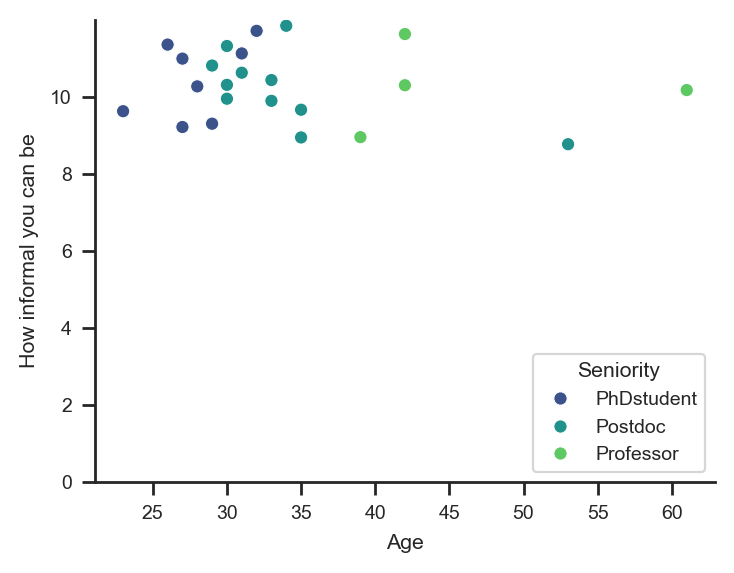
\includegraphics[width=3.82292in,height=2.97917in]{index_files/figure-latex/..-notebooks-example-fig-danish-interaction-output-1.png}

}

\caption{\label{fig-danish-interaction}Figure legends are defined
alongside the figure in the notebook. The figure size in the notebook is
determines its size when embedded in a document 4x3 inches.}

\end{figure}%

As shown in Figure~\ref{fig-meaninformality}, \emph{feugiat leo quis
ante condimentum, eu ornare mauris feugiat. Pellentesque habitant morbi
tristique senectus et netus et malesuada fames ac turpis egestas. Mauris
cursus laoreet ex, ignissim bibendum est posuere iaculis. Suspendisse et
maximus elit. In fringilla gravida ornare. Aenean id lectus pulvinar,
sagittis felis nec, rutrum risus. Nam vel neque eu arcu blandit
fringilla et in quam. Aliquam luctus est sit amet vestibulum eleifend.}

\begin{figure}[H]

\centering{

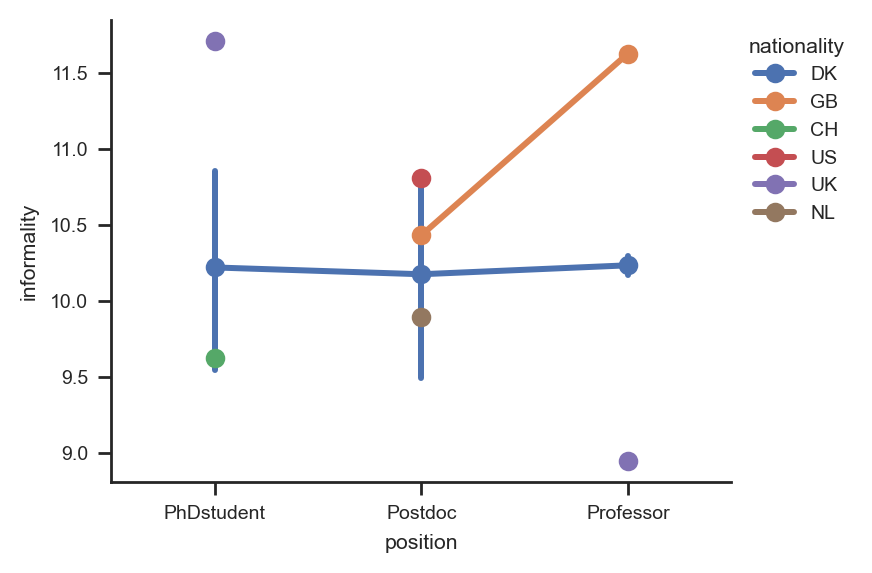
\includegraphics[width=4.54167in,height=2.97917in]{index_files/figure-latex/..-notebooks-example-fig-meaninformality-output-1.png}

}

\caption{\label{fig-meaninformality}Figure legends are defined alongside
the figure in the notebook. The figure size in the notebook is
determines its size when embedded in a document 4x3 inches.}

\end{figure}%

\section{Section (with table embedded from
notebook)}\label{section-with-table-embedded-from-notebook}

\emph{Cubilia hendrerit ipsum suspendisse curae curae suspendisse
scelerisque semper luctus. Erat turpis dictum bibendum taciti pharetra.
Nisi sed vestibulum felis duis; dapibus id. Justo semper felis potenti
commodo class. Mauris venenatis purus integer urna cras faucibus. Eu
consequat varius massa porttitor nisi. Est fringilla sed senectus ante
fames ipsum aenean porta neque,} Table~\ref{tbl-meaninformality} lists
the mean interaction scores by position and nationality.

\begin{longtable}[]{@{}lll@{}}

\toprule\noalign{}
position & nationality & informality \\
\midrule\noalign{}
\endfirsthead
\toprule\noalign{}
position & nationality & informality \\
\midrule\noalign{}
\endhead
\bottomrule\noalign{}
\tabularnewline
\caption{}\label{T_fca36}\tabularnewline
\endlastfoot
Professor & UK & 8.949278 \\
PhDstudent & CH & 9.623167 \\
Postdoc & NL & 9.892308 \\
Postdoc & DK & 10.175595 \\
PhDstudent & DK & 10.220303 \\
Professor & DK & 10.234365 \\
Postdoc & GB & 10.431451 \\
Postdoc & US & 10.808717 \\
Professor & GB & 11.626458 \\
PhDstudent & UK & 11.709714 \\


\caption{\label{tbl-meaninformality}Mean interaction scores by position
and nationality.}

\tabularnewline
\end{longtable}

\emph{Ligula molestie convallis magnis elit tellus volutpat. Hac id in
libero nibh inceptos. Malesuada blandit porttitor ad; netus integer
tortor. Quis venenatis lorem sit ex hendrerit porta in. Purus praesent
felis eget class luctus condimentum finibus quis tincidunt. Nam lectus
malesuada primis dapibus consectetur. Quam placerat nam ullamcorper
fusce conubia fermentum himenaeos gravida nostra.}

\subsection{Discussion}\label{discussion}

\emph{Sociosqu iaculis molestie consectetur; pulvinar imperdiet
pellentesque sollicitudin erat. Varius mattis neque blandit sodales
mauris vestibulum. Iaculis sodales euismod neque risus nostra magna
fermentum eleifend. Tempus consequat montes nec quisque urna quam non
montes. Accumsan ligula mauris nullam nascetur maximus sodales. Non
tellus vel aliquam aenean nulla turpis curabitur potenti. Eleifend
luctus mi primis elementum, rhoncus quisque. Aenean semper blandit
cursus sapien; eget sem. Posuere ultricies torquent tellus ridiculus
enim placerat malesuada tempus.}

\emph{Sapien ullamcorper pretium tellus ultricies sodales aliquet. Proin
eros iaculis fames mus cubilia praesent cubilia. Nulla quam montes sed
varius nullam non. Mi turpis sagittis ornare condimentum consectetur.
Aenean orci sagittis nibh venenatis natoque bibendum semper vel.
Interdum per velit lacus ridiculus augue convallis mollis. Faucibus eget
eros aptent; fusce magnis lacinia duis. Justo ad fames laoreet nisl
viverra.}

\subsection{Conclusion}\label{conclusion}

\emph{Laoreet ullamcorper urna et amet nunc faucibus finibus. Eget
consequat sed integer bibendum a mollis nisl luctus. Orci leo quisque
inceptos imperdiet proin. Pellentesque commodo parturient maecenas eu
leo malesuada ullamcorper nulla viverra. Arcu ligula imperdiet quisque
finibus in curae et accumsan. Egestas gravida sollicitudin venenatis
pellentesque litora leo.}

\emph{Cras velit donec in a morbi ligula, ultrices at tempor. Auctor
lectus in aptent suscipit congue. Urna dui metus risus eleifend odio
nisl magna. Nascetur fringilla metus proin vitae in diam. Class
tincidunt lorem et dictum quisque arcu euismod. Adipiscing dui interdum
aptent fusce pretium pretium. Efficitur imperdiet sem dictumst ultrices
id rhoncus. Congue lacus efficitur scelerisque nibh vestibulum.}

\chapter{Bon mot}\label{bon-mot}

\begin{quote}
Nothing in Biology Makes Sense except in the Light of Evolution

- Theodosius Dobzhansky
\end{quote}

\chapter{References}\label{references}

\phantomsection\label{refs}
\begin{CSLReferences}{1}{0}
\bibitem[\citeproctext]{ref-Dutheil2015}
Dutheil, Julien Y, Kasper Munch, Kiwoong Nam, Thomas Mailund, and Mikkel
H Schierup. 2015. {``{Strong Selective Sweeps on the X Chromosome in the
Human-Chimpanzee Ancestor Explain Its Low Divergence}.''} \emph{PLOS
Genetics} 11 (8): e1005451.
\url{https://doi.org/10.1371/journal.pgen.1005451}.

\bibitem[\citeproctext]{ref-Munch2014}
Munch, Kasper, Thomas Mailund, Julien Y Dutheil, and Mikkel Schierup.
2014. {``{A fine-scale recombination map of the human--chimpanzee
ancestor reveals faster change in humans than in chimpanzees and a
strong impact of GC-biased gene conversion}.''} \emph{Genome Research}
24 (3): 467--74. \url{https://doi.org/10.1101/gr.158469.113}.

\bibitem[\citeproctext]{ref-Nam2015}
Nam, Kiwoong, Kasper Munch, Asger Hobolth, Julien Dutheil, Krishna R
Veeramah, August E Woerner, Michael F Hammer, et al. 2015. {``{Extreme
selective sweeps independently targeted the X chromosomes of the great
apes}.''} \emph{Proceedings of the National Academy of Sciences} 112
(20): 6413--18. \url{https://doi.org/10.1073/pnas.1419306112}.

\bibitem[\citeproctext]{ref-NielsenSlatkin2016}
Nielsen, Rasmgb, and Montgomery Slatkin. 2016. \emph{An Introduction to
Population Genetics: Theory and Applications}.

\bibitem[\citeproctext]{ref-Prufer2012}
Prüfer, Kay, Kasper Munch, Ines Hellmann, Keiko Akagi, Jason R. Miller,
Brian Walenz, Sergey Koren, et al. 2012. {``{The bonobo genome compared
with the chimpanzee and human genomes}.''} \emph{Nature} 486 (7404):
527--31. \url{https://doi.org/10.1038/nature11128}.

\bibitem[\citeproctext]{ref-Skov2023}
Skov, Laurits, Moisès Coll Macià, Elise Anne Lucotte, Maria Izabel Alvez
Cavassim, David Castellano, Mikkel Heide Schierup, and Kasper Munch.
2023. {``{Extraordinary selection on the human X chromosome associated
with archaic admixture}.''} \emph{Cell Genomics}, 100274.
\url{https://doi.org/10.1016/j.xgen.2023.100274}.

\end{CSLReferences}


\backmatter


\end{document}
